\documentclass[a4paper,11pt]{article}

\usepackage{a4wide}
\usepackage{hyperref}

\usepackage{amsmath,bm}
\newcommand{\td}{\mathrm{d}}
\newcommand{\te}{\mathrm{e}}
\newcommand{\ti}{\mathrm{i}}
\newcommand{\sinc}{\mathrm{sinc}}
\newcommand{\sign}{\mathrm{sign}}
\newcommand{\atan}{\mathrm{atan}}
\usepackage{tikz}

\title {Analytical integrals of kernels}

\begin{document}

\maketitle

\tableofcontents

\section{Analytical integrals of the Laplace kernel}

This section describes the analytical formulae used to integrate the kernel of the Laplace equation in two dimensions over straight lines.

The kernel is defined as
%
\begin{equation}
G({\bf y}, {\bf x}) = -\frac{\ln |{\bf y}-{\bf x}|}{2\pi} = -\frac{\ln r}{2\pi}
\end{equation}
%
where ${\bf x}$ is the source point. The kernel exhibits a weak (integrable) singularity when $r \to 0$.

The kernel's normal derivative with respect to the normal  ${\bf n}_y$ at coordinate ${\bf y}$ can be formulated as
%
\begin{equation}
G'_{n_y}({\bf y}, {\bf x}) = \frac{\td G(r)}{\td r} \frac{\partial r}{\partial n_y} = -\frac{1}{2\pi r} \frac{{\bf r} \cdot {\bf n}_y}{r} = -\frac{({\bf y}-{\bf x}) \cdot {\bf n}_y}{2\pi r^2}
\end{equation}
%
this derivative kernel contains a strong singularity and can be integrated in a CPV sense.

The kernel's second derivative tensor is expressed as
%
\begin{equation}
	G''_{ij} = \left(G'_j\right)'_i
	= \frac{-1}{2\pi}\left(\frac{r_j}{r^2}\right)'_i
	= \frac{-1}{2\pi r^2}\left( \delta_{ij} - 2\frac{r_j}{r} \frac{r_i}{r}\right)
\end{equation}

As a consequence, the second normal derivative is expressed as
%
\begin{equation}
	G''_{n_x n_y}({\bf x}, {\bf y})
	= -n_{xi} G''_{ij} n_{yj}
	=  \frac{1}{2\pi r^2} \left( n_{xi} n_{yi} - 2\frac{n_{xi} r_i}{r} \frac{r_j n_{yj}}{r}\right)
\end{equation}


\subsection{Collocation}

The following parts describe the case of collocation where ${\bf x}={\bf x}_0$ is a fixed location and integration is performed with respect to the variable ${\bf y}$. In general, the integrals are written in the form
%
\begin{equation}
\int_S K({\bf y}, {\bf x}_0) N({\bf y}) \td S_y
\end{equation}
%
where $K$ denotes one of the kernels introduced above, and $N({\bf y})$ denotes (polynomial) weighting functions over the element.

\subsubsection{Regular integrals}

\begin{figure}
\center
\begin{tikzpicture}[scale=1]
\small
\draw [thin, ->] (2,1) -- (3,.5) node [right] {$\xi$};
\draw [thin, ->] (2,1) -- (2.5,2) node [left] {$\eta$};
\path [draw, fill] (3,3) circle(.05) node [right] {${\bf x}_0$};
\path [draw, very thick, fill] (4,0) circle(.05) node [below] {${\bf y}_2$} -- (4.5,-.25) circle(.05) node [below] {${\bf y}$} -- (6,-1) circle(.05) node [below] {${\bf y}_1$};
\path [draw, thick, ->] (5,-.5) -- (5.5,.5) node [above] {${\bf n}$};
\end{tikzpicture}
\caption{Coordinate transform for the definition of the regular integrals over the straight line element}
\label{fig:regular_local}
\end{figure}

In order to define the regular integrals in a convenient way local coordinates are introduced, as shown in Fig.~\ref{fig:regular_local}:
%
\begin{align}
\xi &= ({\bf y} - {\bf x}_0) \cdot {\bf t} \qquad {\bf t} = \frac{{\bf y}_1 - {\bf y}_2}{|{\bf y}_1 - {\bf y}_2|} \nonumber \\
\eta &= ({\bf x}_0 - {\bf y}) \cdot {\bf n}
\end{align}
%
The straight line element lies in the $\eta = 0$ line. The nodal locations ${\bf y}_1$ and ${\bf y}_2$ correspond with the local coordinates $\xi_1$ and $\xi_2$, respectively, and due to the proper selection of the normal's direction, $\xi_1 = \xi_2 + d$ where $d$ is the element length. The origin of the local system is the image of ${\bf x}_0$ on the element's line.

The regularity of the integrals is ensured if $\eta \ne 0$ or $\sign \xi_1 = \sign \xi_2$


\paragraph{SLP kernel}

The regular integral of the single layer potential kernel can be now written in the general form
%
\begin{align}
I &= \frac{-1}{2\pi} \int_{\xi_2}^{\xi_1} \ln\left(\sqrt{\xi^2+\eta^2}\right) \left(a_0 + a_1 \xi + a_2 \xi^2\right) \td \xi \\
 &= \frac{1}{2\pi} \left[
\left(\frac{1}{9} - \frac{\ln \rho}{3}\right) a_2 \xi^3
+ \frac{a_1}{2} \left(\frac{\xi^2}{2}
- \rho^2 \ln \rho\right)
- a_0 \xi \ln \rho
+ \left(\frac{a_2 \eta^2}{3} - a_0 \right) \left(\eta \atan\frac{\xi}{\eta} - \xi\right)
\right]_{\xi_2}^{\xi_1} \nonumber
\end{align}
%
where $\rho = r = \sqrt{\xi^2+\eta^2}$.

\paragraph{DLP kernel}

For the case of the double layer potential kernel, the integral is transformed as
%
\begin{equation}
I = \frac{-1}{2\pi} \int_{\xi_2}^{\xi_1} \frac{-\eta \left(a_0 + a_1 \xi + a_2 \xi^2 \right)}{\xi^2+\eta^2}\td \xi
= \frac{1}{2\pi} \left[
\left( a_0 - a_2 \eta^2\right) \atan \frac{\xi}{\eta} + \left(a_2 \xi + a_1 \ln r\right) \eta
\right]_{\xi_2}^{\xi_1}
\end{equation}

\paragraph{HSP kernel}

For the case of the HSP kernel, let $n_{\xi}$ and $n_{\eta}$ denote the normal at $x_0$ in the local frame of reference. In this case the integral is expressed as
%
\begin{equation}
I
= \int_{\xi_2}^{\xi_1} G''_{n_x n_y} \td \xi
= -\frac{1}{2\pi} \left[ \frac{ \eta n_{\xi} + \xi n_{\eta} }{\rho^2} \right]_{\xi_2}^{\xi_1}
\end{equation}

\subsubsection{Constant line SLP}

\begin{align}
\int_{S} G({\bf y}, {\bf x}) \td y
& = \frac{-1}{2\pi}\lim_{\epsilon \to 0}
\left( \int_{-d_1}^{-\epsilon} \ln |y| \td y + \int_{\epsilon}^{d_2}  \ln |y| \td y \right) \nonumber \\
& = \frac{-1}{2\pi}\lim_{\epsilon \to 0}
\left( \int_{\epsilon}^{d_1} \ln y \td y + \int_{\epsilon}^{d_2}  \ln y \td y \right) \nonumber \\
&=
\frac{d_1(1-\ln d_1) + d_2(1-\ln d_2)}{2\pi}
\end{align}

\subsubsection{Constant line DLP}

\begin{equation}
\int_{S} G'_{n_y}({\bf y}, {\bf x}) \td y = 0
\end{equation}
%
as the element normal is perpendicular to the distance ${\bf y}-{\bf x}$.

\subsubsection{Constant line HSP}

First approach: finite part integral
%
\begin{align}
\int_{S} G''_{n_x n_y}({\bf y}, {\bf x}) \td y
&= \frac{1}{2\pi} \lim_{\epsilon \to 0} \left(\int_{-d_1}^{-\epsilon} \frac{1}{y^2}\td y + \int_{\epsilon}^{d_2} \frac{1}{y^2} \td y\right) \nonumber \\
&= \frac{1}{2\pi} \lim_{\epsilon \to 0} \left(\left[\frac{-1}{y}\right]_{-d_1}^{-\epsilon} +  \left[\frac{-1}{y}\right]_{\epsilon}^{d_2} \right)
\nonumber \\
&= \frac{-1}{2\pi} \left(\frac{1}{d_1} +  \frac{1}{d_2} \right) + \lim_{\epsilon \to 0} \frac{1}{\pi\epsilon}
\end{align}


Second approach: approaching the boundary:
%
\begin{align}
\frac{\partial}{\partial n_x}
\int_{-d_1}^{d_2} 
\frac{\partial}{\partial n_y}
\frac{-\ln |r|}{2\pi}
\td y 
&=
\frac{\partial}{\partial z}
\int_{-d_1}^{d_2} 
\frac{-1}{2\pi r} \frac{(y, -z) \cdot (0,1)}{r}
\td y \nonumber \\
&=
\frac{1}{2\pi} \frac{\partial}{\partial z}
\int_{-d_1}^{d_2} 
\frac{z}{\left(y^2+z^2\right)}
\td y \nonumber \\
&=
\frac{1}{2\pi} \frac{\partial}{\partial z}
\left[
\tan^{-1}\left(d_2/z\right)
-
\tan^{-1}\left(-d_1/z\right)
\right]
\nonumber \\
&=
\frac{1}{2\pi} \frac{\partial}{\partial z}
\left[
\tan^{-1}\left(d_2/z\right) + \tan^{-1}\left(d_1/z\right)
\right]
\nonumber \\
&=
\frac{1}{2\pi} 
\left[
\frac{-d_2}{d_2^2+z^2} + \frac{-d_1}{d_1^2+z^2}
\right]
\nonumber \\
& \to
\frac{-1}{2\pi} 
\left[
\frac{1}{d_2} + \frac{1}{d_1}
\right]
\end{align}


\subsection{Galerkin}

\subsubsection{Face match}

\paragraph{Constant line SLP}

\begin{equation}
\int_{0}^{d}
\lim_{\epsilon \to 0}
\left(
\int_{0}^{x-\epsilon} G(x-y) \td y
+
\int_{x+\epsilon}^{d} G(x-y) \td y
\right)
\td x
=
d^2\frac{3-2\ln d}{4\pi}
\end{equation}

\paragraph{Linear line SLP}

\begin{equation}
\int_{0}^{d} N_i(x) \int_{0}^{d} G(x-y) N_j(y) \td y \td x
=
\frac{d^2}{32\pi} \begin{bmatrix}
7-4 \ln d & 5 - 4 \ln d \\
5-4 \ln d & 7 - 4 \ln d
\end{bmatrix}
\end{equation}

\subsubsection{Edge match}

The local coordinate system used for the calculation of edge-match type singular integrals is shown in Fig.~\ref{fig:local_galerkin_edge}. The lengths of the elements are denoted with $d_1$ and $d_2$, and the second element defines the direction of the normal vector. The angle between the two elements is denoted by $\phi$.

\begin{figure}
\center
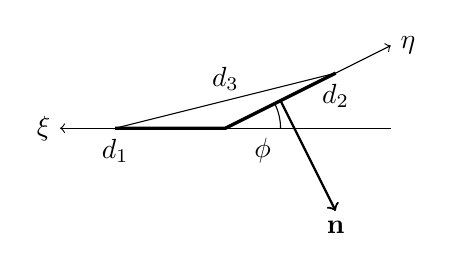
\begin{tikzpicture}[scale=.7]
\path [draw, ->] (3,0) -- (-3,0) node [left] {$\xi$};
\path [draw, ->] (0,0) -- (3,1.5) node [right] {$\eta$};
\path [draw] (-2,0) --  node [above] {$d_3$} (2,1);
\path [draw, very thick] (-2,0) node [below] {$d_1$} -- (0,0) -- (2,1) node [below] {$d_2$};
\path [draw, thick, ->] (1,.5) -- (2,-1.5) node [below] {${\bf n}$};
\draw [domain=0:26.5] plot ({cos(\x)}, {sin(\x)});
\path (1,0) node [below left] {$\phi$};
\end{tikzpicture}
\caption{Local coordinates for the definition of Galerkin edge-match singular integrals}
\label{fig:local_galerkin_edge}
\end{figure}

\paragraph{Constant line SLP}

\begin{multline}
\int_{S_{x}} \int_{S_{y}} G(r) \td S_y \td S_x =
\int_{0}^{d_1} \int_{0}^{d_2}
\frac{-1}{2\pi}\ln \sqrt{(\xi+\eta \cos\phi)^2 + (\eta\sin\phi)^2}
\td \eta \td \xi \\
=
\frac{1}{4 \pi}
\left[
d_1 d_2 \left(3 - 2 \ln d_3 \right)
+ \cos\phi \left(d_1^2 \ln \frac{d_1}{d_3} + d_2^2 \ln \frac{d_2}{d_3}\right)
- \sin\phi \left(d_1^2 q\left(\frac{d_2}{d_1}, \phi\right) + d_2^2 q\left(\frac{d_1}{d_2}, \phi\right)\right)
\right]
\end{multline}
%
where
%
\begin{equation}
q(a, \phi) = \atan\left(\frac{a}{\sin\phi} + \cot\phi\right) - \atan\left(\cot\phi\right)
\end{equation}

\paragraph{Constant line DLP}

\begin{align}
\int_{S_{x}} \int_{S_{y}} G'(r) r'_{n_{y}} \td S_y \td S_x
&=
\frac{-1}{2\pi}\int_{0}^{d_1} \int_{0}^{d_2}
\frac{\xi\sin\phi}{(\xi+\eta \cos\phi)^2 + (\eta\sin\phi)^2}
\td \eta \td \xi \nonumber \\
&=
\frac{1}{2\pi}\left[
	d_2 \cos\phi q\left(\frac{d_1}{d_2}, \phi\right)
	- d_1 q\left(\frac{d_2}{d_1}, \phi\right)
	+ d_2 \sin\phi \ln \frac{d_2}{d_3}
\right]
\end{align}



\section {Analytical integrals of the 2D Helmholtz kernel}

\subsection{Introduction}

The kernel is defined as
%
\begin{equation}
G({\bf y}, {\bf x}) = \frac{-\ti}{4} H_0^{(2)}(kr), \quad r = |{\bf y} - {\bf x}|
\end{equation}
%
where ${\bf x}$ is the source point. The kernel exhibits a weak (integrable) singularity when $r \to 0$.

\subsection{Basic properties}

The Hankel function may be written as
%
\begin{equation}
H_0^{(2)}(z) = J_0(z) - \ti Y_0(z)
\end{equation}
%
and the small argument series expansion of the involved Bessel functions around $z=0$ are
%
\begin{align}
J_0(z) &= \sum_{n=0}^{\infty} (-1)^n \frac{\left(\frac{z}{2}\right)^{2n}}{\left(n!\right)^2} \\
Y_0(z) &= \frac{2}{\pi}
\sum_{n=0}^{\infty} (-1)^n \left(\log \frac{z}{2} + \gamma - C_n \right) \frac{\left(\frac{z}{2}\right)^{2n}}{\left(n!\right)^2}
\end{align}
%
where $\gamma$ denotes Euler's constant and $C_n$ denotes the harmonic sum
%
\begin{equation}
C_0 = 0, C_n = C_{n-1} + \frac{1}{n}
\end{equation}



\subsection{Collocation}

\paragraph{Constant line SLP}

The integral to evaluate can be simplified to the form
%
\begin{equation}
I = \frac{-\ti}{4} \int_{-R}^R  H_0^{(2)}(kr)  \td y
\end{equation}
%
where $R$ denotes the element's half length.

From the above series expansions, the integral $I$ may be expressed in terms of the following integral elements ($D = 2R$):
%
\begin{align}
\int_{-R}^R
\left(\frac{kr}{2}\right)^{2n} \td y
= D \left( \frac{kR}{2} \right)^{2n} F_n \\
\int_{-R}^R
\log \frac{kr}{2} \cdot \left(\frac{kr}{2}\right)^{2n} \td y
= D \left(\frac{kR}{2}\right)^{2 n} G_n
\end{align}
%
where
%
\begin{align}
F_n &= \frac{1}{2n+1} \\
G_n &= \frac{\log\frac{kR}{2}} {2 n + 1} - \frac{1}{(2 n + 1)^2}
\end{align}


\subsection{Galerkin}

\subsubsection{Face match}

\paragraph{Constant line SLP}

The integral to evaluate can be simplified to the form
%
\begin{equation}
I = \frac{-\ti}{4} \int_{-R}^{R} \int_{-R}^R  H_0^{(2)}(k|y-x|)  \td y \td x
\end{equation}
%
where $R$ denotes the element's half length.

From the above series expansions, the integral $I$ may be expressed in terms of the following integral elements ($r=|y-x|$, $D = 2R$):
%
\begin{align}
\int_{-R}^{R} \int_{-R}^R  \left(\frac{kr}{2}\right)^{2n}  \td y \td x
= D^2 \cdot (kR)^{2n} F_n
\\
\int_{-R}^{R} \int_{-R}^R  \log \frac{kr}{2} \cdot \left(\frac{kr}{2}\right)^{2n}  \td y \td x
= D^2 \cdot (kR)^{2n} G_n
\end{align}
%
where
%
\begin{align}
F_n &= \frac{1}{(n+1)(2n+1)}
\\
G_n &= \begin{cases}
\log kR - \frac{2}{3} & n = 0 \\
\frac{\log kR}{(n+1)(2n+1)} - \frac{4n+3}{2(n+1)^2(2n+1)^2}& n > 0
\end{cases}
\end{align}

As a result, the total integral is expressed as
%
\begin{equation}
I = -\ti R^2
\sum_{n=0}^{\infty} (-1)^n \frac{(kR)^{2n}}{\left(n!\right)^2}
\left(
F_n
- \frac{2 \ti}{\pi}
\left(G_n + \left(\gamma - C_n \right) F_n \right)
\right)
\end{equation}


\end{document}

